Cominciamo con lo sviluppare singolarmente ogni entità fondamentale in modo da approfondirne le caratteristiche principali. Quindi dalla visione generale entriamo nello specifico seguendo l'approccio misto precedentemente citato.\newline

\subsubsection{RICHIESTA SUL MEPA}
Il concetto di Richiesta sul MePA raggruppa due entità, che sono il tipo di richiesta con cui la nostra azienda si interfaccia. In questo caso si parla di richieste di offerta sotto forma di Gara Pubblica oppure di Trattativa diretta.\newline In entrambi i casi abbiamo un numero univoco associato alla richiesta di offerta che la identifica, dobbiamo avere dei parametri fondamentali associati alla richiesta, che sono il limite di spesa specificato, il codice IPA e l'offerta proposta dalla nostra azienda a scopo statistico e le date di inizio e termine offerta.\newline
La richiesta sotto forma di gara pubblica avrà anche l'aggiudicatario della gara e la sua offerta, mentre il trattativa diretta dovrà definire se la trattativa è andata attraverso il valore stipulata, riferendosi al contratto di vendita.\newline 
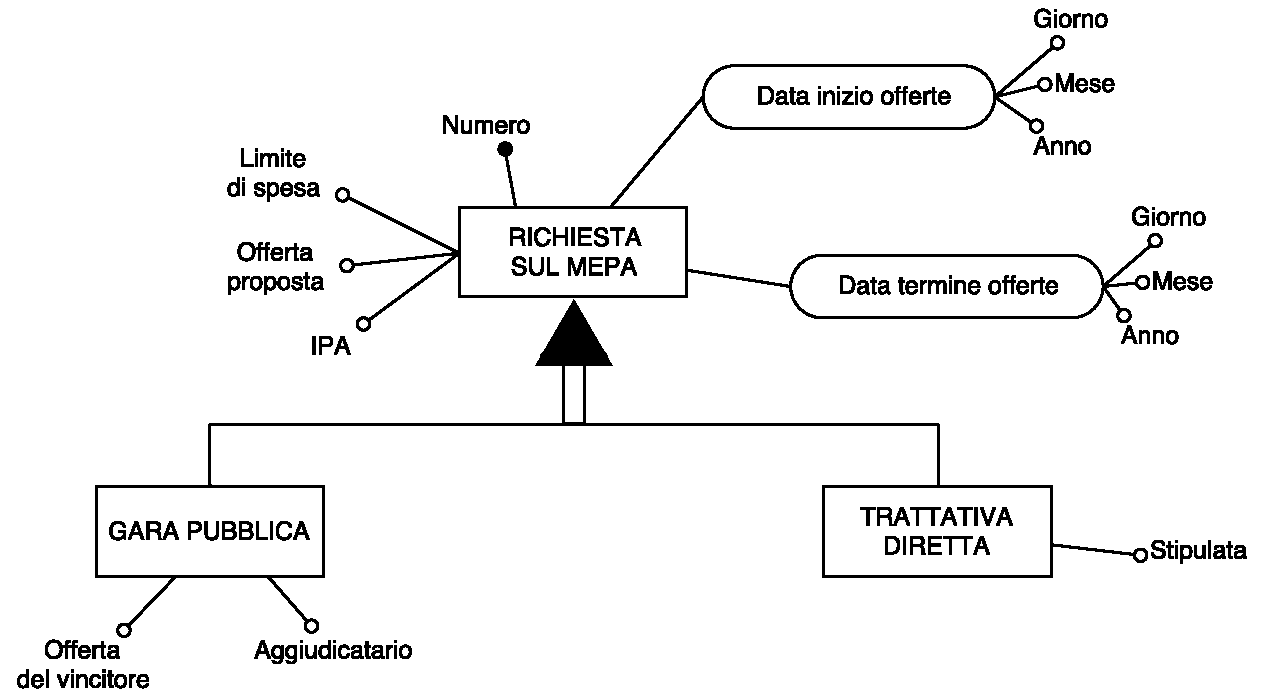
\includegraphics[width=0.7\linewidth]{./immagini/richiesta_sul_mepa.pdf}

\subsubsection{PA O PERSONA O AZIENDA}
Questa entità raggruppa appunto le entità che hanno relazioni commerciali con la nostra azienda. Concettualmente c'è una doppia divisione, infatti l'entità fondamentale si divide in due entità quali il Fornitore e il Cliente. A sua volta l'entità cliente si divide in Pubblica Amministrazione, l'entità di maggior interesse, intorno alla quale si costruisce l'entità di Richiesta sul MEPA precedentemente descritta, e l'entità Privato, che è invece un cliente ordinario che può essere una persona o un'azienda.\newline
Tutte queste entità hanno bisogno di un codice identificativo, il codice PA nel caso delle pubbliche amministrazioni, il codice fiscale per le persone o la partita IVA per le aziende. In più viene tenuto in considerazione l'indirizzo pubblico PEC e la ragione sociale che contiene i dati dell'indirizzo (via, numero civico, città, CAP) e dati personali(nome, telefono, email).\newline
Vicino al fornitore è riportata l'entità dei costi di spedizone che non ha nulla a che fare con l'identità generale di pa, azienda o persona, ma è strettamente correlata al fornitore e va considerata, portando con se i dati riguardo il costo della spedizione, il peso e la somma delle misure massima e i tempi di consegna.
\newline
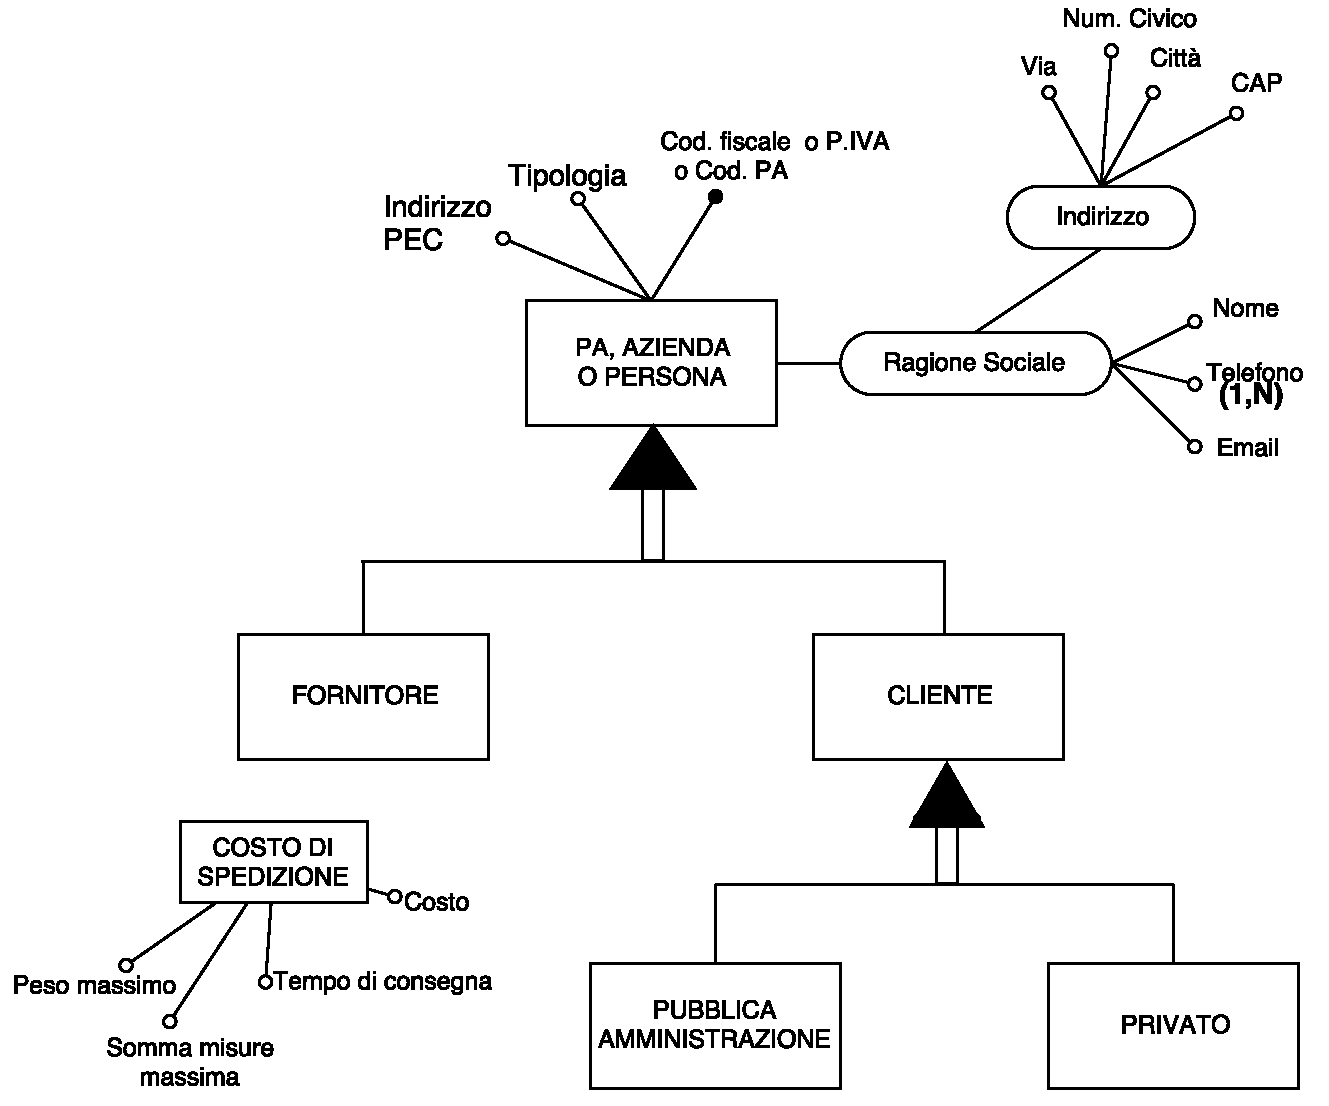
\includegraphics[width=0.7\linewidth]{./immagini/pa_persona_o_azienda.pdf}

\subsubsection{PRODOTTO O SERVIZIO}
Questa identità raggruppa due identità molto diverse, il Prodotto e il Servizio, ed ha in comune soltanto il codice identificativo associato al prodotto al servizio.\newline
Il prodotto è a sua volta un entità che ne raggruppa molte altre, in particolare tutti i prodotti disponibili (Notebook, Memoria di Massa, RAM, Stampante, PC Desktop, Monitor, Cartuccia d'Inchiostro, Toner). Tutti questi prodotti devono avere indicati il produttore, il modello, le dimensioni e il peso, poi in base al prodotto in questione ognuno ha caratteristiche diverse rappresentate nei suoi attributi.\newline
D'altra parte il servizio è un entità singola particolare in quanto tra i suoi attributi ha il costo del servizio emesso e la tipologia, che devo descrivere la prestazione effettuata. A tal proposito la descrizione del servizio deve essere standardizzata e necessità di particolare attenzione in quanto il servizio è solitamente descritto in maniera non univoca. \newline
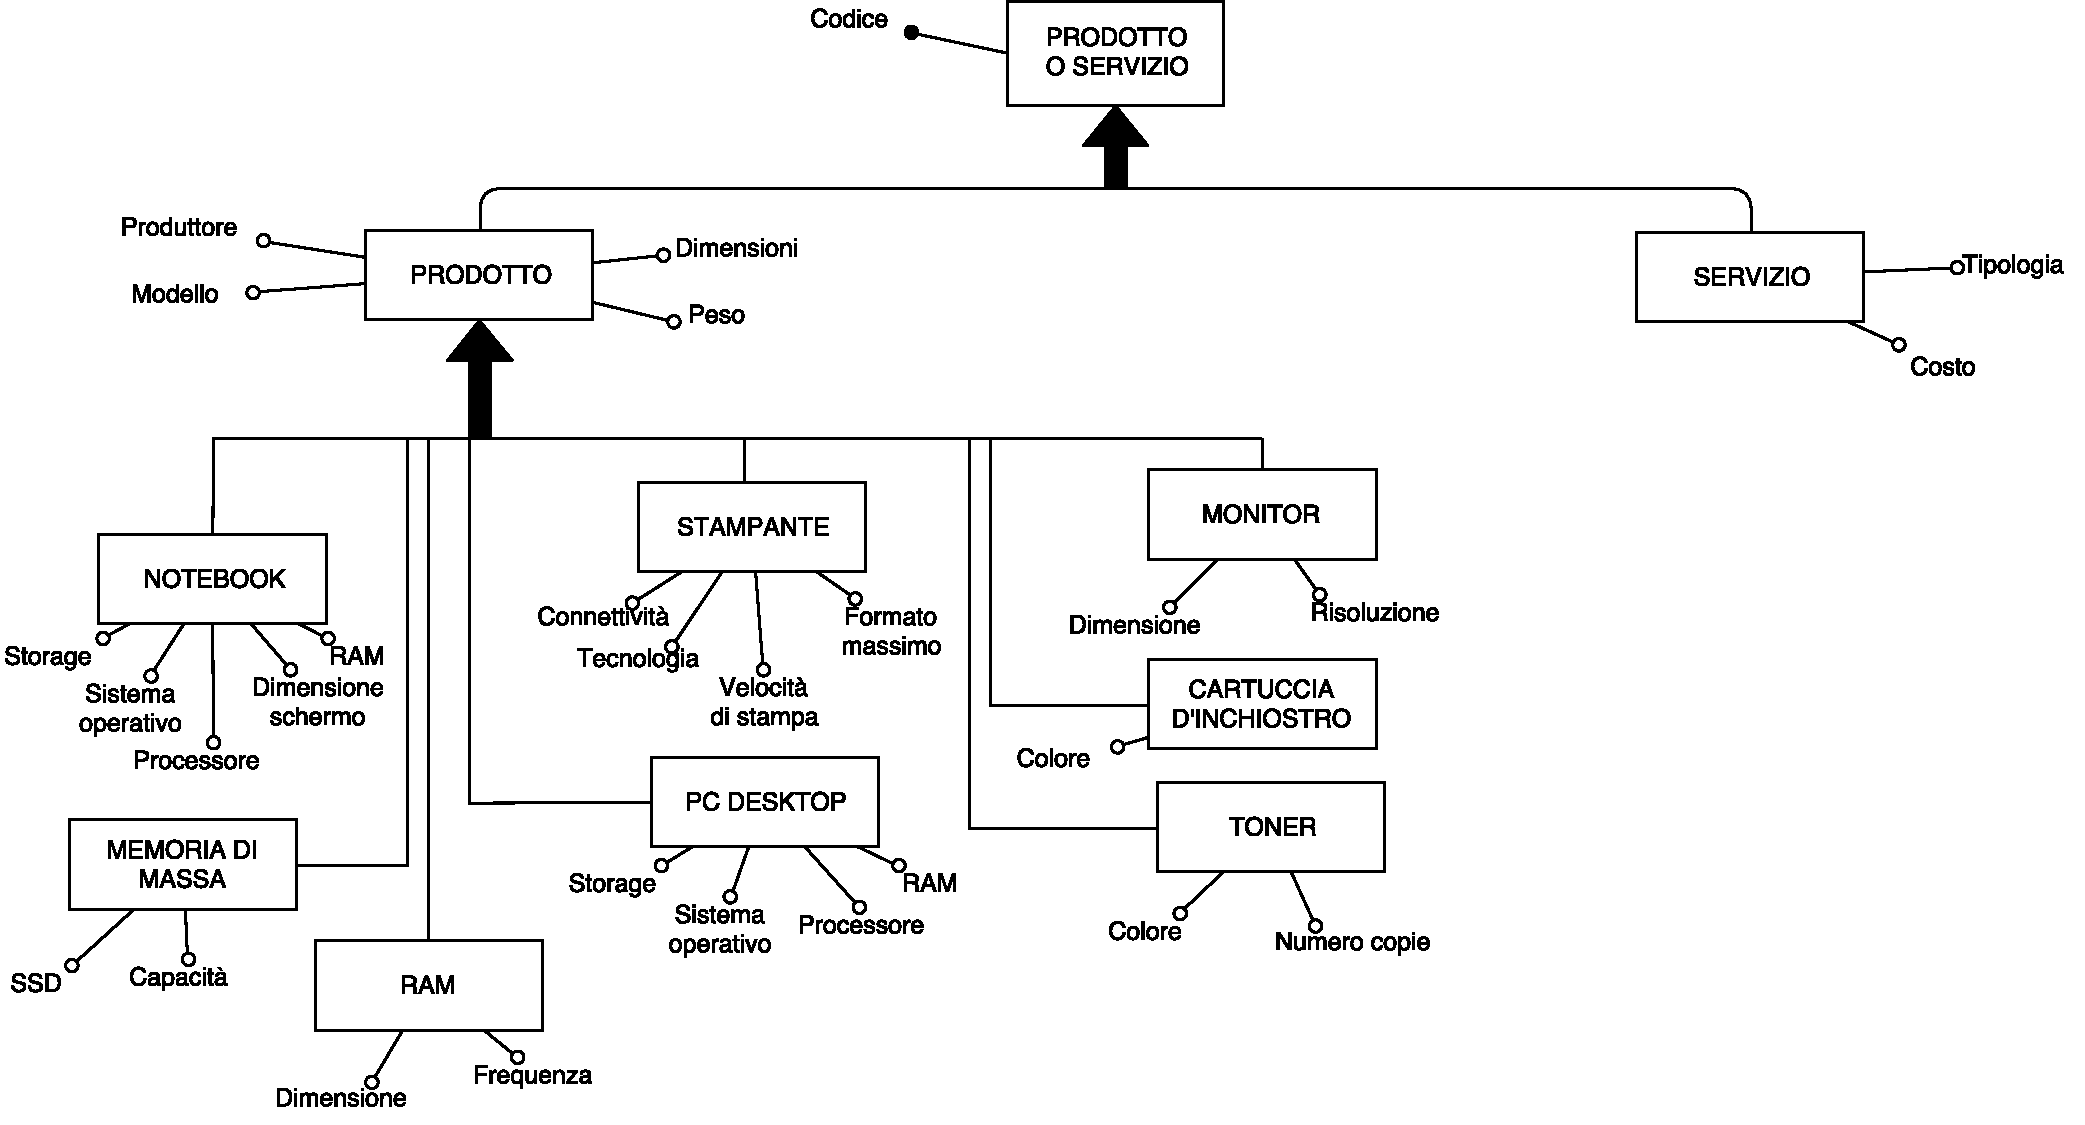
\includegraphics[width=0.7\linewidth]{./immagini/prodotto_servizio.pdf}

\subsubsection{FATTURA}
L'entità della Fattura ha un ruolo centrale in quando ad essa sono collegate tutte le operazioni effettuate dall'azienda, quindi acquisto dai fornitori oppure la vendita a privati o pubbliche amministrazioni.\newline
La fattura è identificata da un codice univoco, e le sue specifiche sono l'importo, l'emittento e il destinatario della fattura. In più sono riportate data di emissione, data di scadenza e data di pagamento.\newline
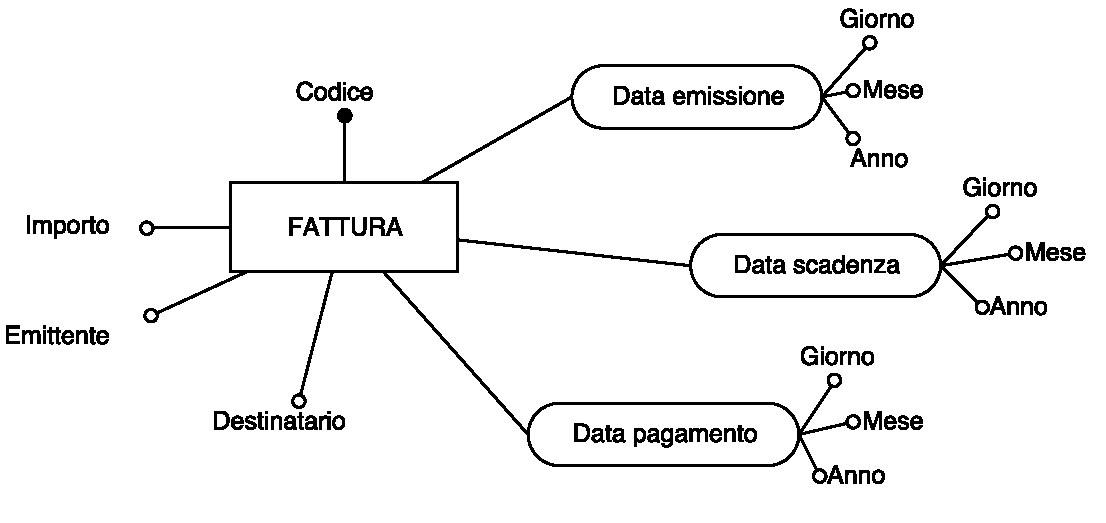
\includegraphics[width=0.7\linewidth]{./immagini/fattura.pdf}



% Procediamo ora secondo la strategia Top-down raffinando le definizioni delle entità e aggiungendo ulteriori relazioni.
% \subsubsection{Personaggio}
% Sappiamo che il personaggio ha parecchie caratteristiche e valori che lo contraddistinguono, possiamo suddividerle in 4 gruppi:
% Posizione, Fisico, Statistiche e Statistiche totali
%
% \begin{figure}[H]
% \centering
% 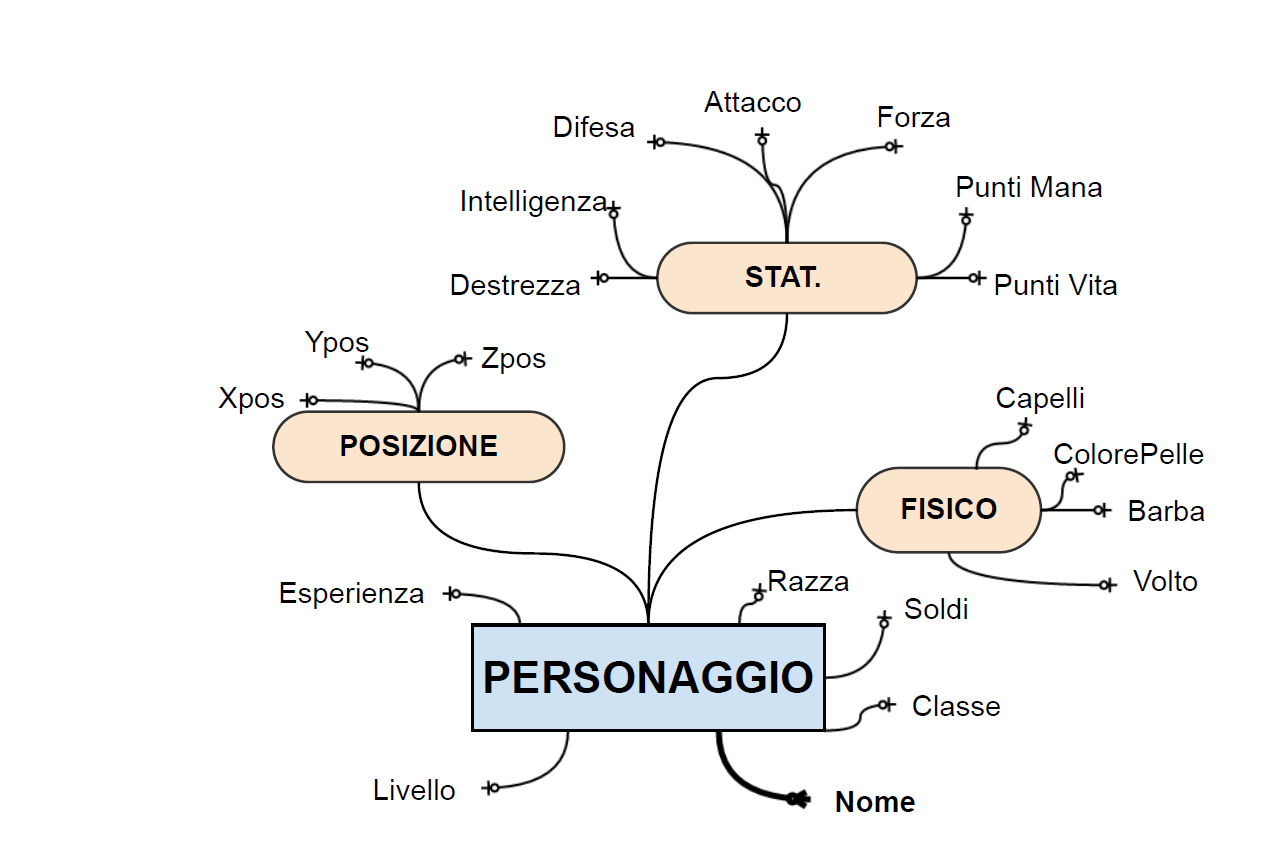
\includegraphics[width=0.7\linewidth]{./immagini/personaggiodef.png}
% \end{figure}
%
% \newpage
%
%
% \subsubsection{NPC}
% Gli npc sono divisi principalmente in ostili e amichevoli, questo ne determina fortemente la funzione all'interno del gioco, le relazioni con le altre entità nonchè i dati stessi che essi utilizzano, è quindi necessaria una Generalizzazione che i suddivida di conseguenza
%
% \begin{figure}[H]
% \centering
% 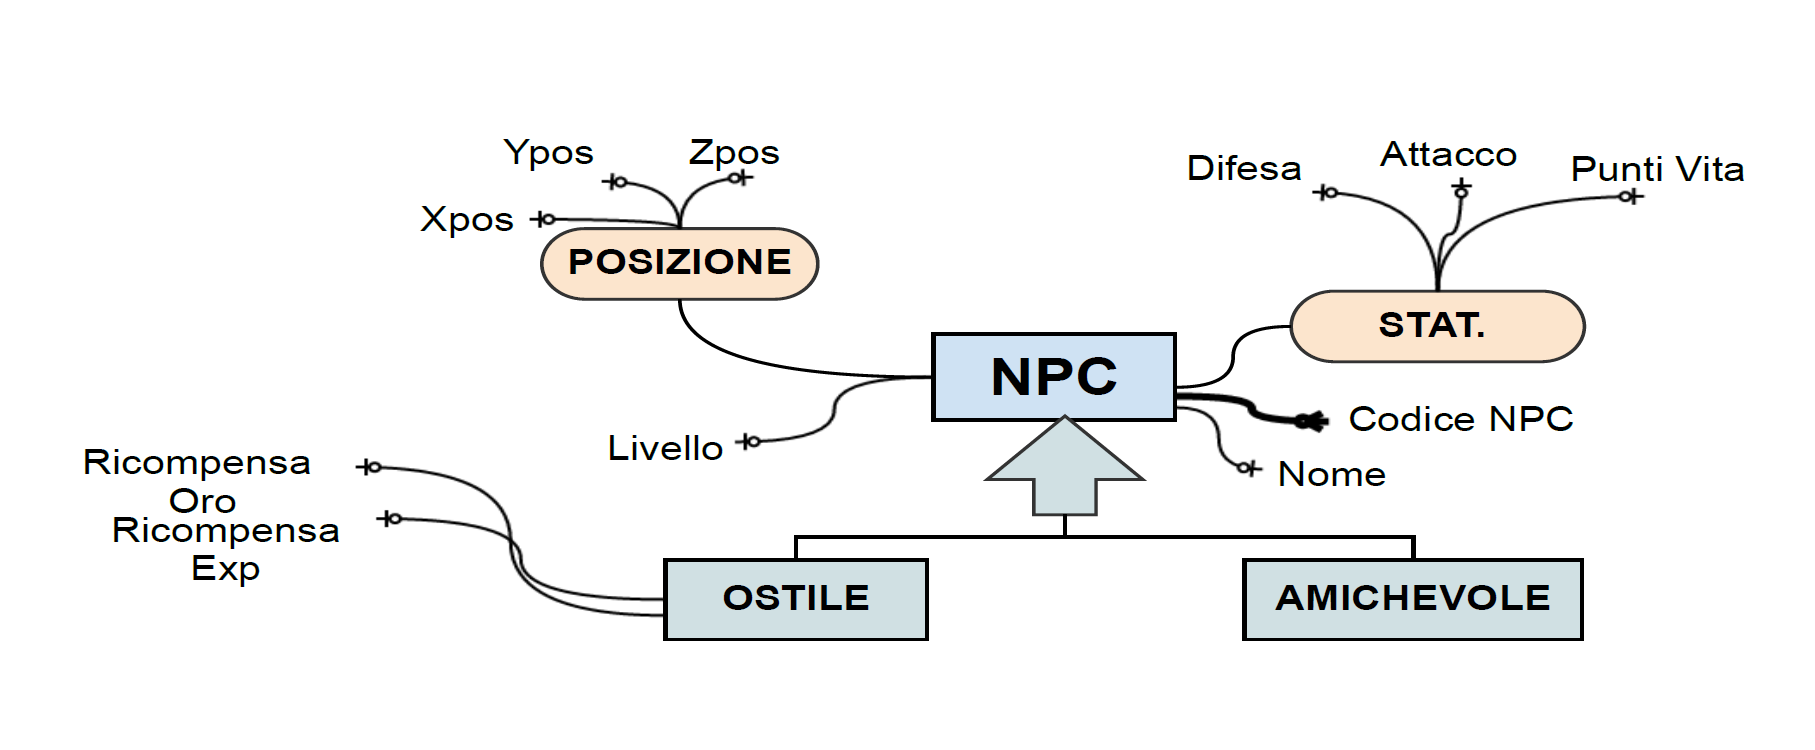
\includegraphics[width=0.7\linewidth]{./immagini/npcdef.png}
% \end{figure}
%
%
% \subsubsection{Oggetto}
% Per gli oggetti sappiamo che alcuni di essi possono essere equipaggiati, consumati dal personeggio oppure essere oggetti missione, questo fatto oltre a comportare una Generalizzazione implica la necessità di una relazione di equipaggiamento, una di consumo e una di stock per descrivere la proprietà di un OGGETTO da parte di un PERSONAGGIO
%
% \begin{figure}[H]
% \centering
% 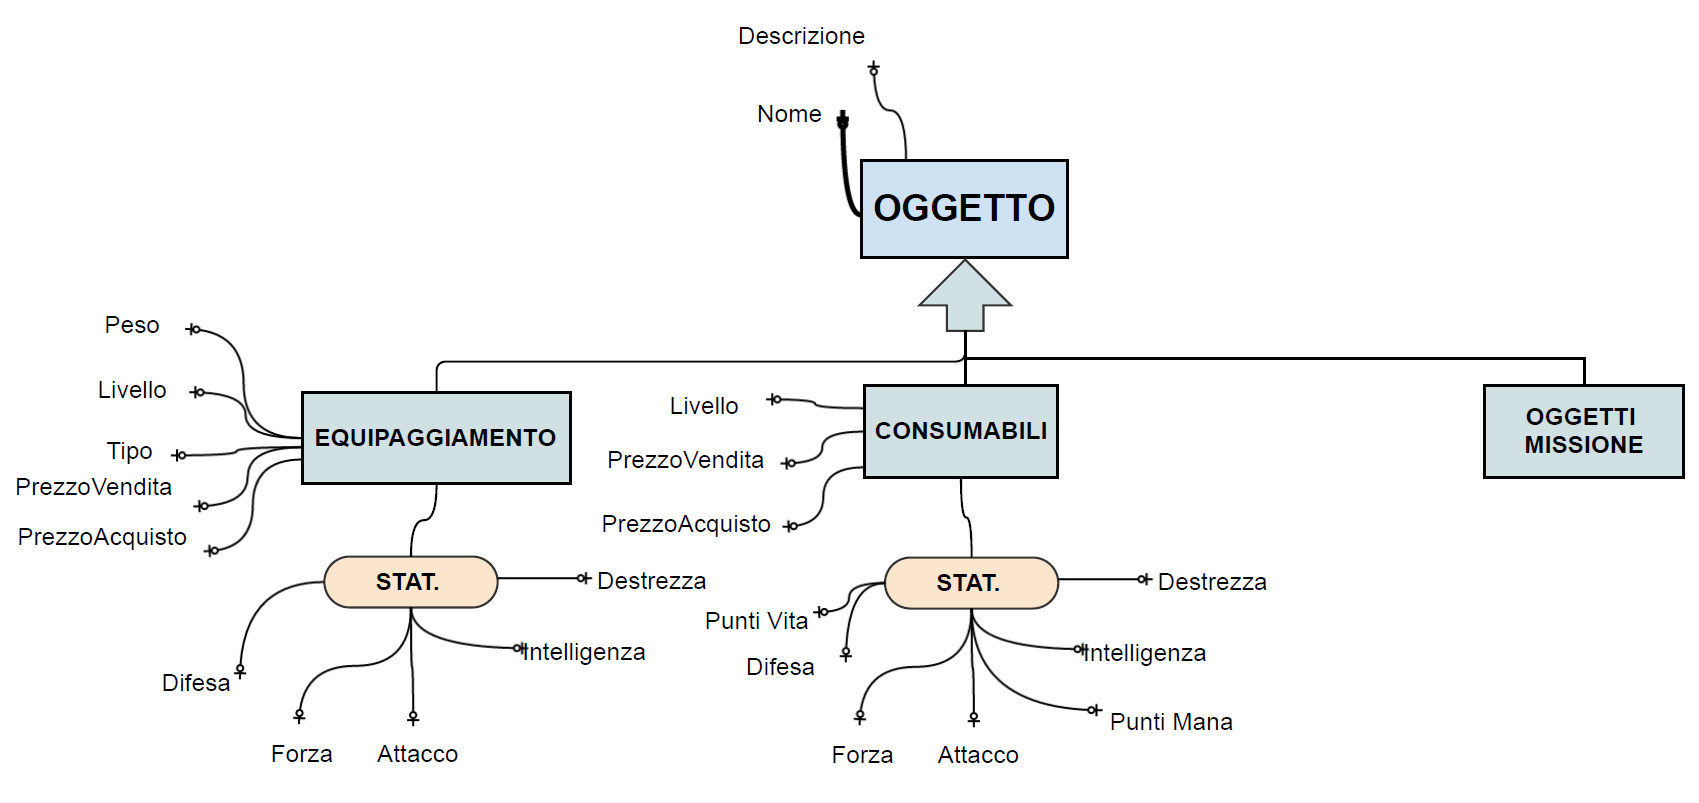
\includegraphics[width=0.7\linewidth]{./immagini/oggettodef.png}
% \end{figure}
%
%  \newpage
%
% \subsubsection{Abilità}
% Dalle interviste sappiamo che le abilità hanno svariati attributi che sono poi i valori da sommare alle statistiche dei personaggi che imparano le abilità, hanno anche un costo e un livello massimo.
%
% \begin{figure}[H]
% \centering
% 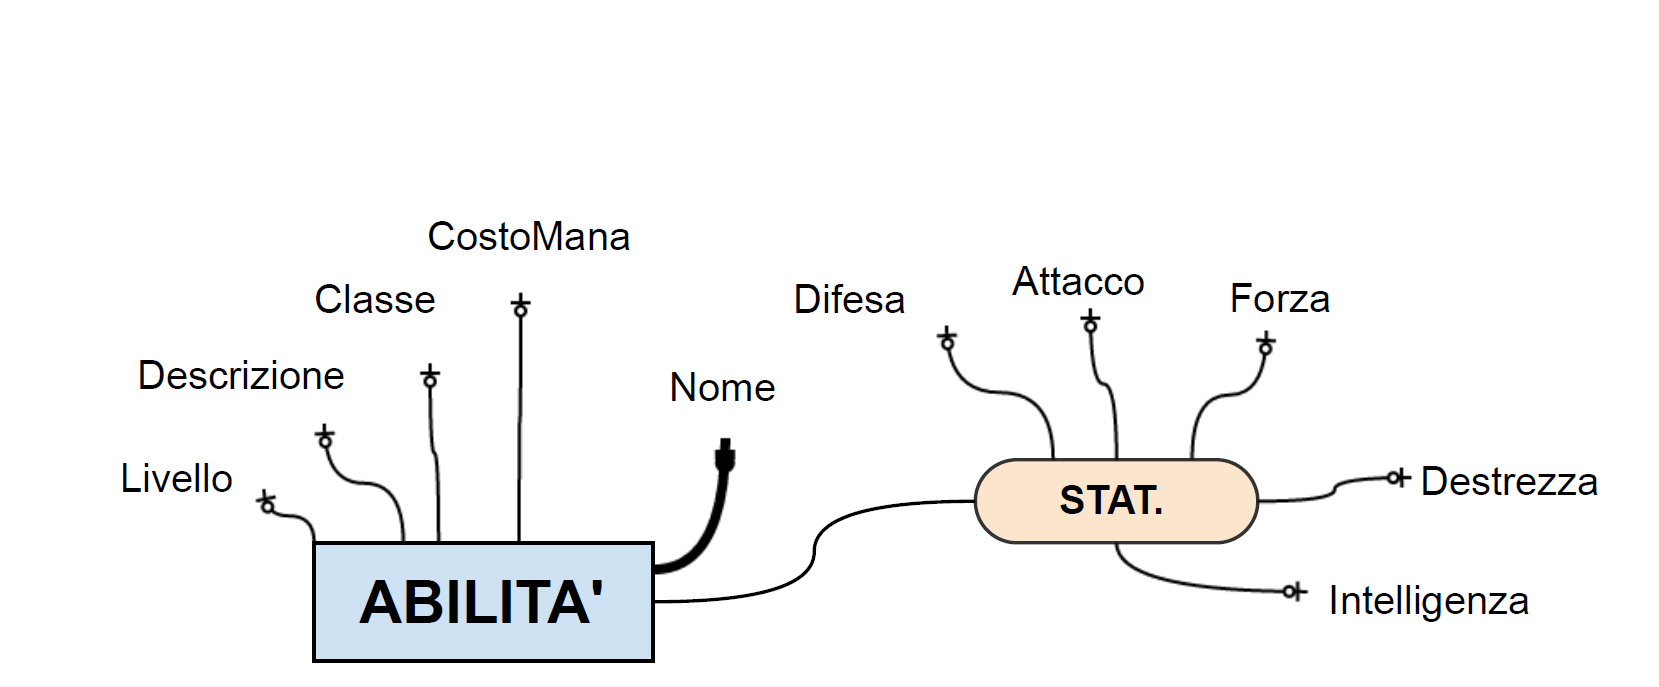
\includegraphics[width=0.7\linewidth]{./immagini/ABILITADEF.png}
% \end{figure}
%
% \subsubsection{Transazione}
% Le transazioni saranno necessarie solo per tenere traccia degli acquisti della sessione, esse avranno un SOGGETTO e un OGGETTO intesi come "chi vende a chi compra"
%
% \begin{figure}[H]
% \centering
% 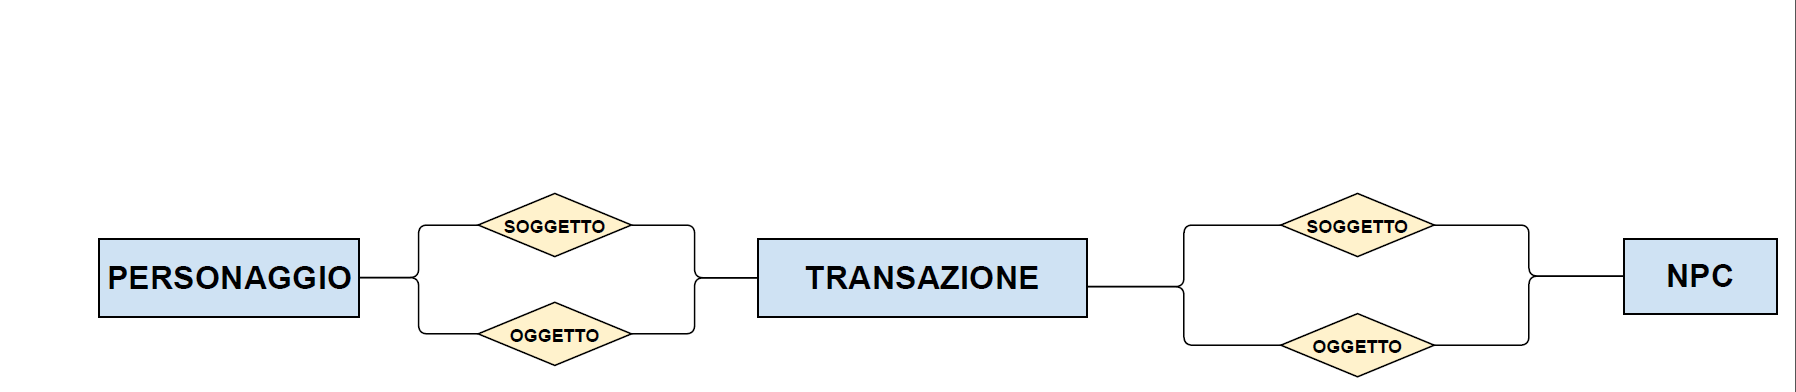
\includegraphics[width=0.7\linewidth]{./immagini/TRANSAZ.png}
% \end{figure}
% AMBIGUITA
%
% \subsubsection{Utente}
% L'utente è la persona vera e propria che si logga per giocare con uno dei suoi personaggi, puo fare acquisti nello Store con una delle sue carte di credito, eliminare o creare personaggi e modificare i suoi dati di fatturazione.
%
%
% \begin{figure}[H]
% \centering
% 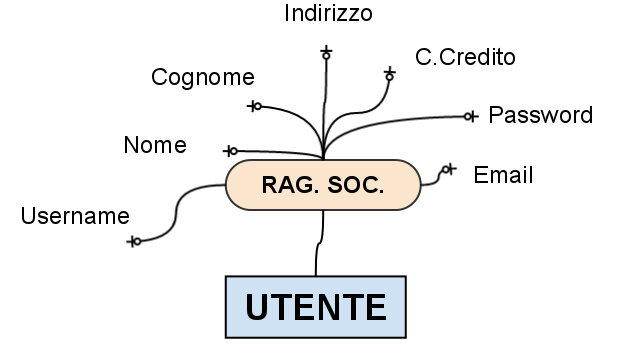
\includegraphics[width=0.7\linewidth]{./immagini/untentedef.png}
% \end{figure}
%
% \subsubsection{Prodotto}
% I PRODOTTI nel nostro gioco sono principalmente 3, cioè le SOTTOSCRIZIONI, I PACCHETTI OGGETTI che permettono di acquistare un gruppo di oggetti Elencati e le ESPANSIONI del Gioco che permettono di raggiungere un livello massimo piu alto.
%
% \begin{figure}[H]
% \centering
% 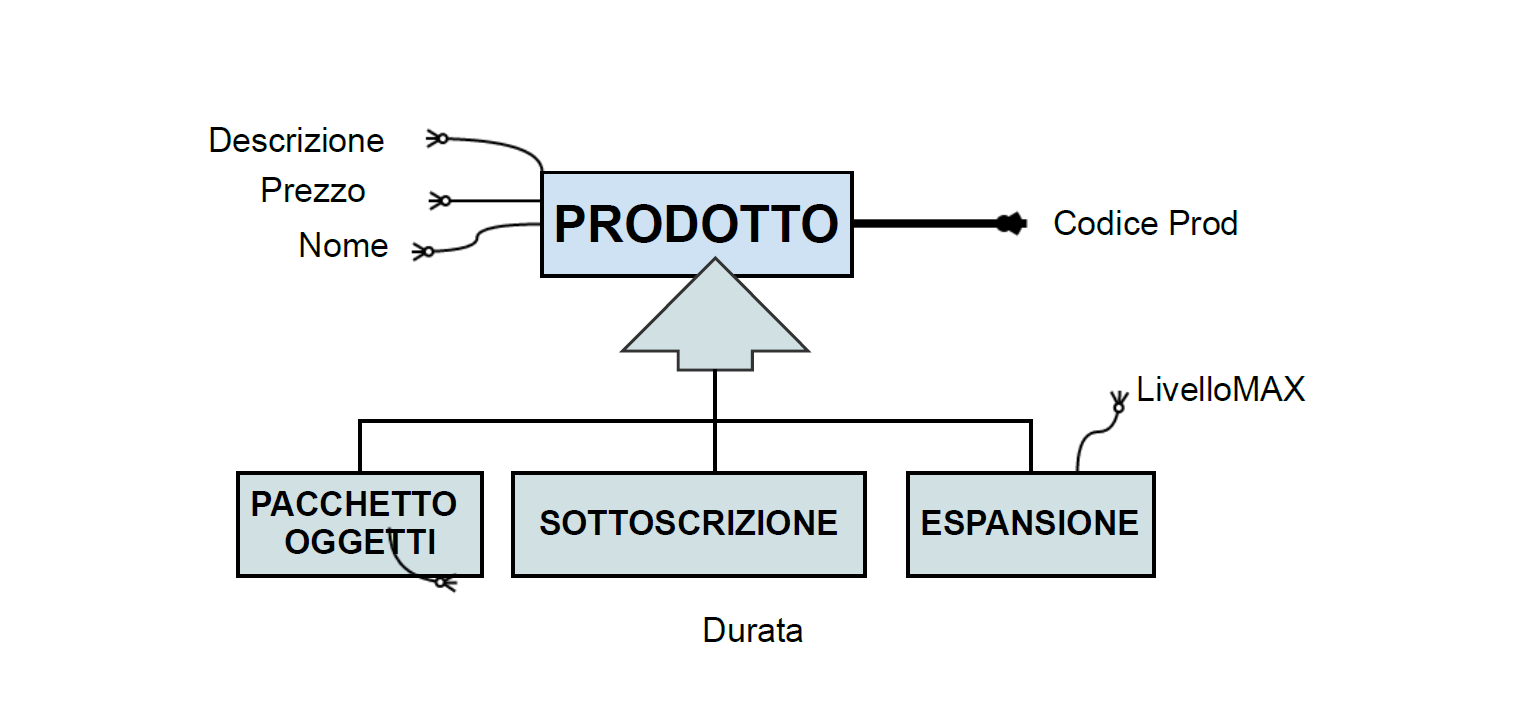
\includegraphics[width=0.7\linewidth]{./immagini/prodottodef.png}
% \end{figure}
%
% \newpage
